\chapter{Sequence modeling}


\section{Memoryless approach}
\marginnote{Memoryless approach}

Neural network that takes as input a fixed number of elements of the sequence.

\begin{remark}
    They are not ideal for long-term dependencies.
\end{remark}



\section{Recurrent neural network}

\begin{description}
    \item[Recurrent neural network (RNN)] \marginnote{Recurrent neural network}
        Neural network in which hidden states have backward connections in such a way that each state depends on the past history.

        Inputs are processed one time step at a time as they cannot be parallelized since each step needs the hidden state at the previous time step.

        \begin{figure}[H]
            \centering
            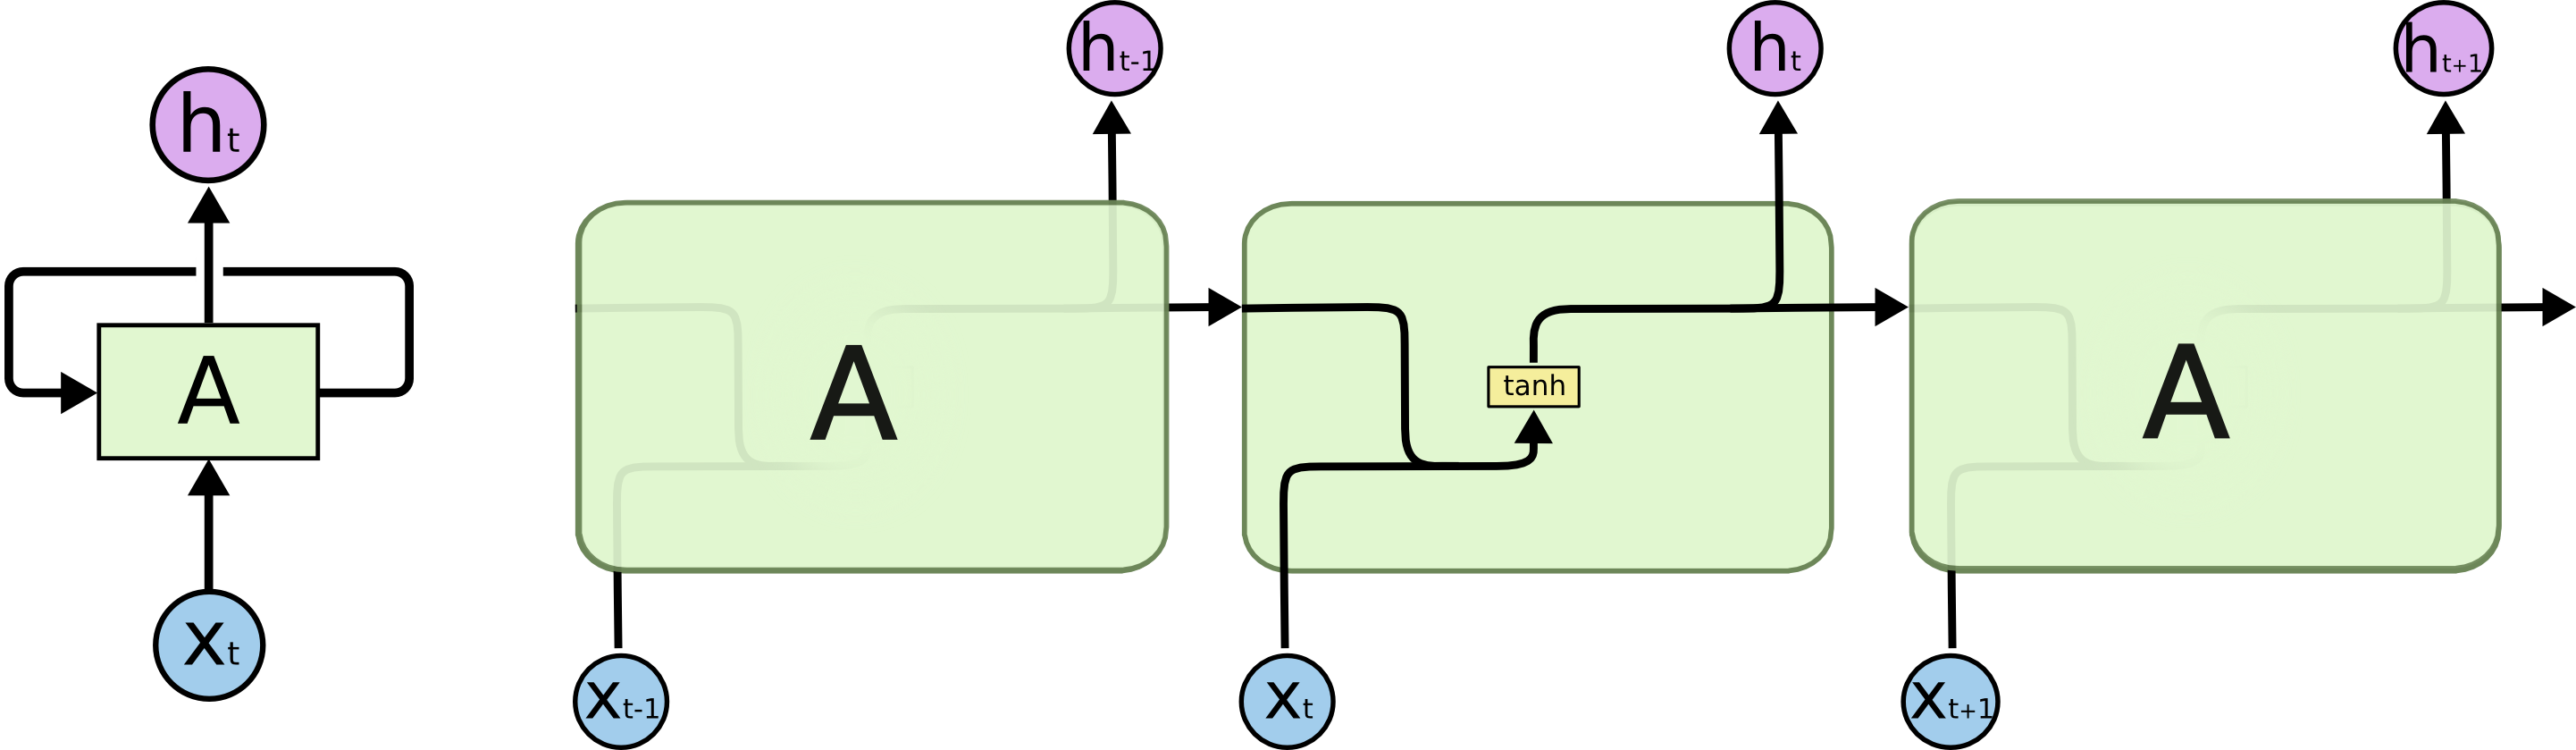
\includegraphics[width=0.65\linewidth]{./img/rnn.png}
            \caption{Example of RNN (left) and its unfolded version (right)}
        \end{figure}

    \item[Backpropagation] \marginnote{RNN backpropagation}
        Weight updates in RNNs are computed by averaging the gradients of each time step (i.e. a forward pass involves processing an entire sequence).

        By seeing an RNN in its unfolded form, this way of updating the weights guarantees that the parameters of the network remain the same for each time step.

        \begin{remark}
            For long sequences, it is very easy for the gradient to explode or vanish.
        \end{remark}

    \item[Hidden state initialization] \marginnote{Hidden state initialization}
        There are different ways to set the initial hidden state at $t=0$:
        \begin{itemize}
            \item Initialize to zero.
            \item Sample from a known distribution.
            \item Learned during training.
        \end{itemize}
\end{description}



\subsection{Long-short term memory}
\marginnote{Long-short term memory}

Traditional RNNs usually only carry to the next time step the output of the current step.

Long-short term memory is an architecture of RNN that, along side the output of the previous layer, allows the model itself to learn what to "remember".

\begin{figure}[H]
    \centering
    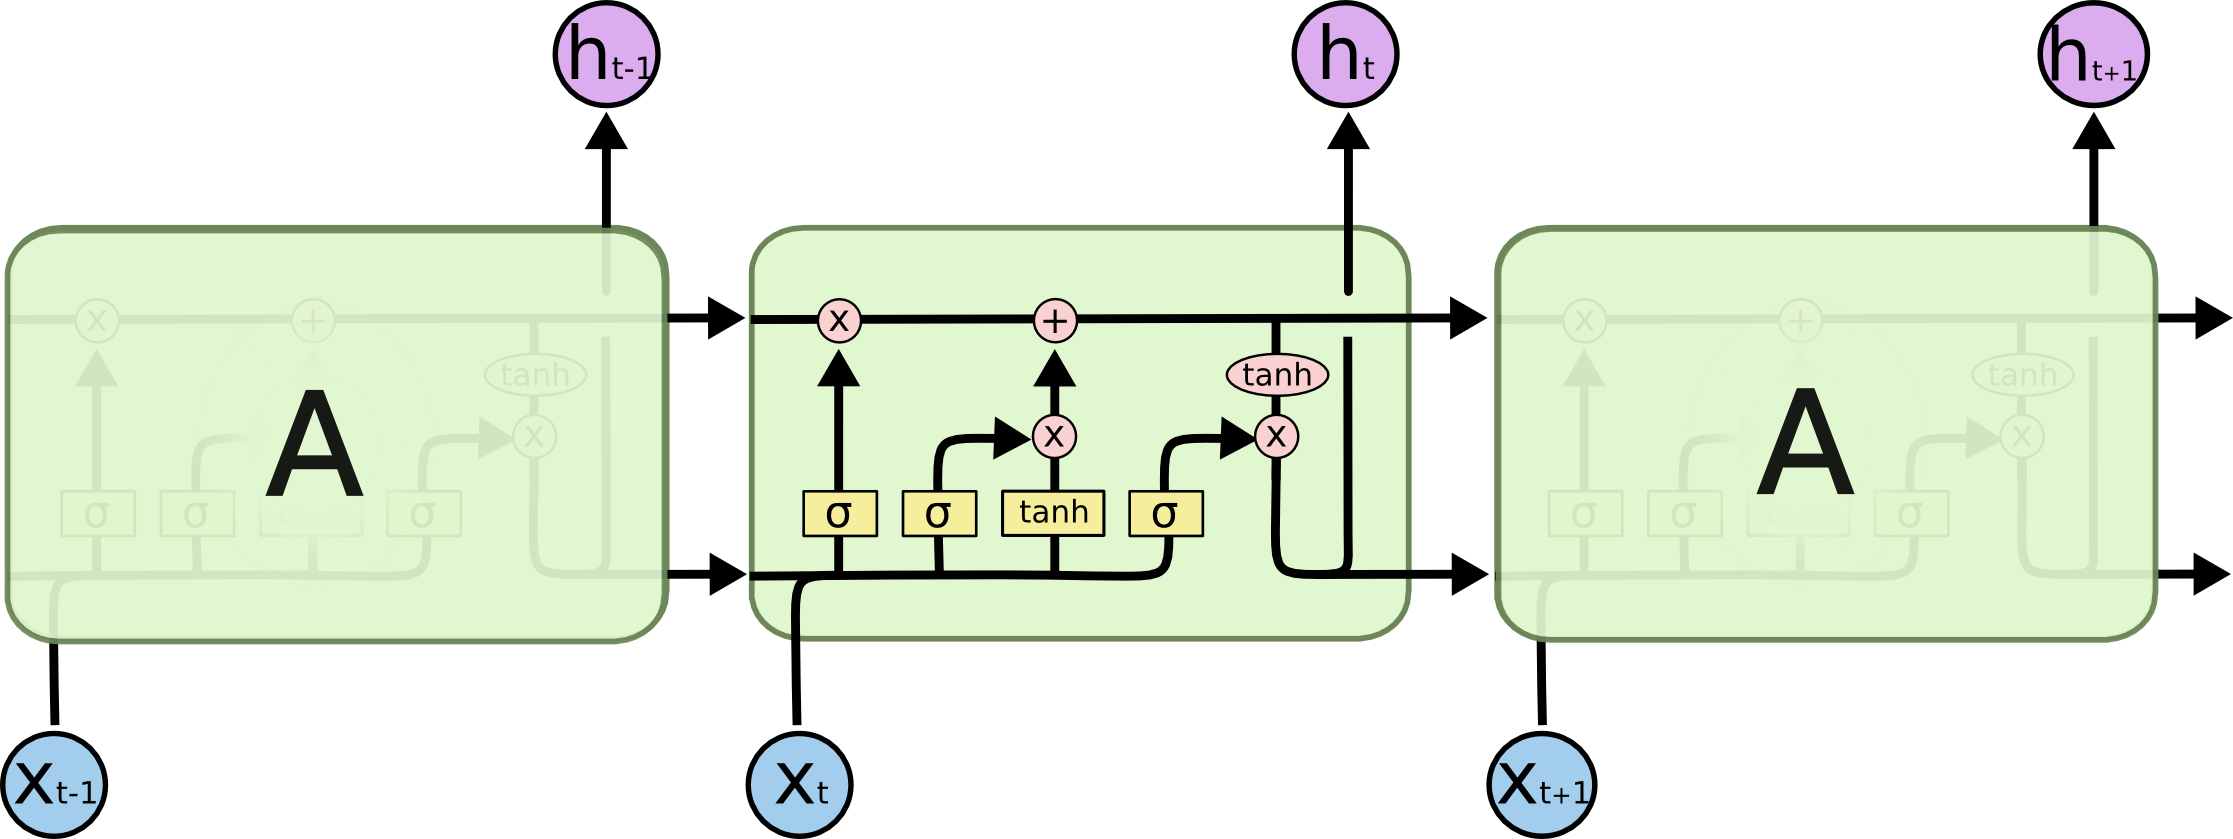
\includegraphics[width=0.6\linewidth]{./img/lstm.png}
\end{figure}


Let:
\begin{itemize}
    \item $W_g$ and $b_g$ be the weights and biases of the component $g$,
    \item $h_t$ the output of at time step $t$,
    \item $x_t$ the input at time step $t$,
\end{itemize}
an LSTM has the following components:
\begin{descriptionlist}
    \item[Forget gate] 
        Computes a mask $f_t$ that will decide which part of the memory to preserve.\\
        \begin{minipage}{0.6\linewidth}
            \[ f_t = \sigma( W_f \cdot [h_{t-1}, x_t] + b_f) \]
        \end{minipage}
        \begin{minipage}{0.35\linewidth}
            \centering
            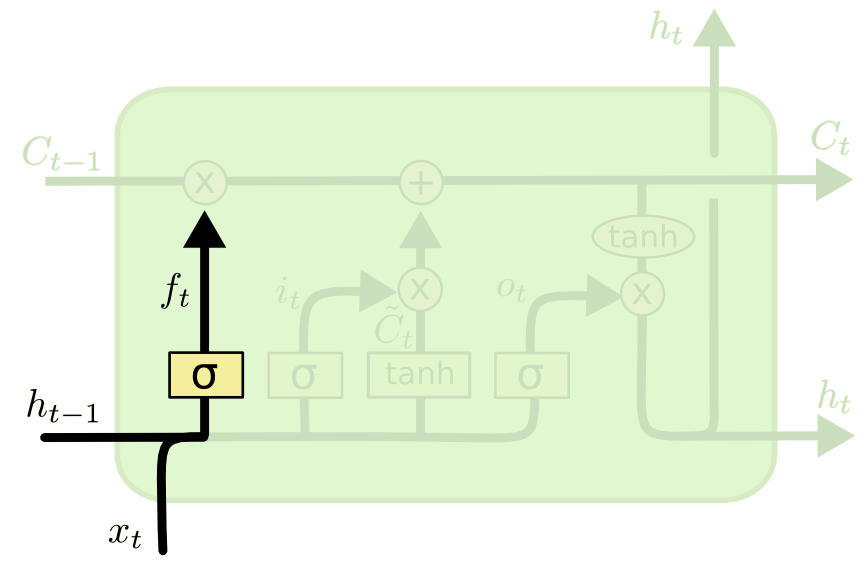
\includegraphics[width=0.85\linewidth]{./img/forget_gate.png}
        \end{minipage}

    \item[Update gate] 
        It is composed of two parts:
        \begin{descriptionlist}
            \item[Input gate] Computes a mask $i_t$ that decides which part of the input to preserve.
            \item[\texttt{tanh} layer] Creates a vector $\tilde{C}_t$ of new candidate values to potentially be saved in the memory.
        \end{descriptionlist}
        \begin{minipage}{0.6\linewidth}
            \[
                \begin{split}
                    i_t &= \sigma( W_i \cdot [h_{t-1}, x_t] + b_i) \\
                    \tilde{C}_t &= \texttt{tanh}( W_C \cdot [h_{t-1}, x_t] + b_C) \\
                \end{split}
            \]
        \end{minipage}
        \begin{minipage}{0.35\linewidth}
            \centering
            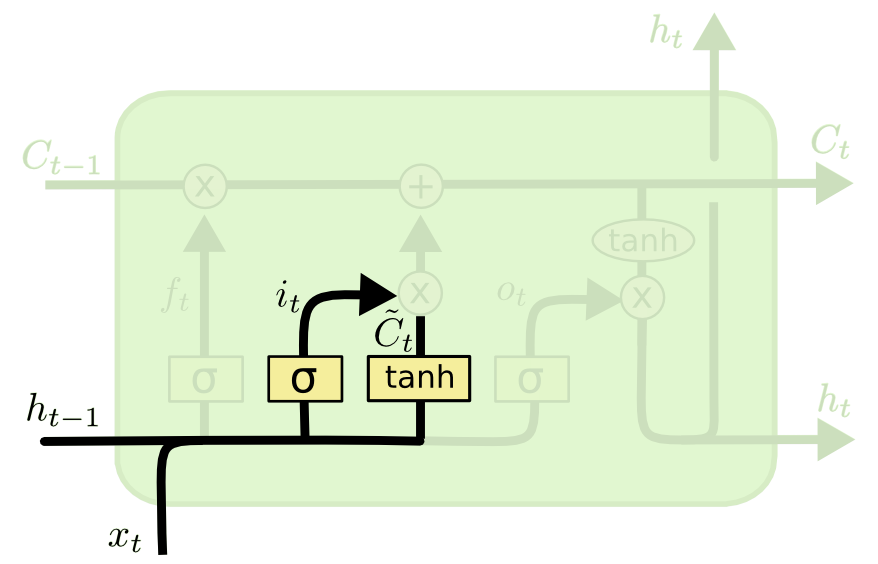
\includegraphics[width=0.85\linewidth]{./img/update_gate.png}
        \end{minipage}

    \item[C-line] 
        Represents the memory of the network.
        At each step, the memory $C_{t-1}$ of the previous step is updated and a new state $C_t$ is outputted to the next step.\\
        \begin{minipage}{0.6\linewidth}
            \[ C_t = f_t * C_{t-1} + i_t * \tilde{C}_t \]
        \end{minipage}
        \begin{minipage}{0.35\linewidth}
            \centering
            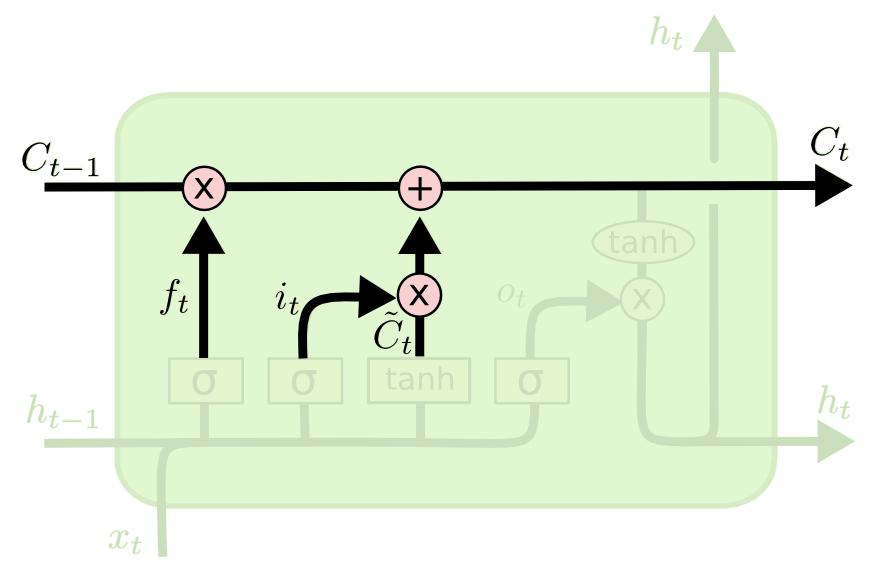
\includegraphics[width=0.85\linewidth]{./img/cline_update.png}
        \end{minipage}

    \item[Output gate] 
        The output $h_t$ at step $t$ is determined by the current input and the updated memory.\\
        \begin{minipage}{0.6\linewidth}
            \[
                \begin{split}
                    o_t &= \sigma( W_o \cdot [h_{t-1}, x_t] + b_o) \\
                    h_t &= o_t * \texttt{tanh}(C_t) \\
                \end{split}
            \]
        \end{minipage}
        \begin{minipage}{0.35\linewidth}
            \centering
            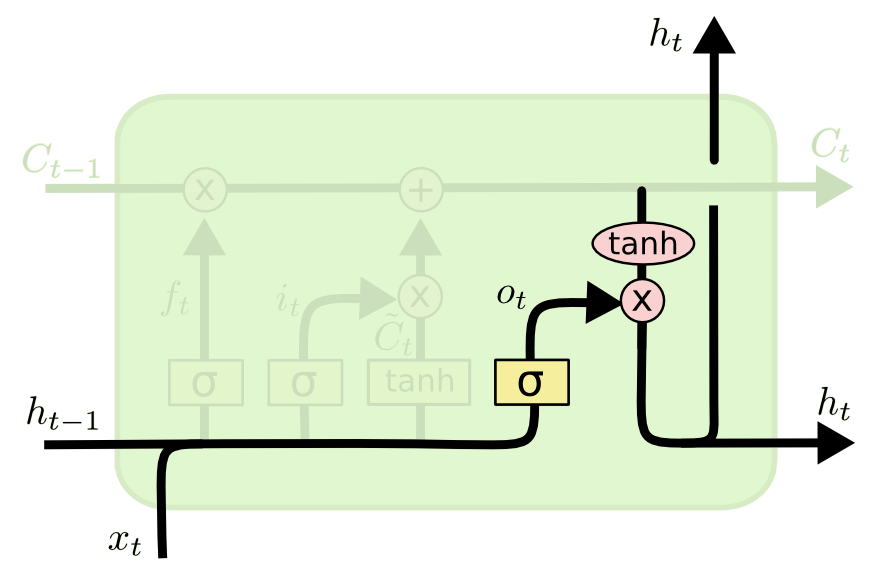
\includegraphics[width=0.85\linewidth]{./img/output_gate.png}
        \end{minipage}
\end{descriptionlist}


\section{Transformers}


\begin{description}
    \item[Attention] \marginnote{Attention}
        Capability of a model to focus on specific parts of the input.
        Attention can be implemented through different approaches:
        \begin{description}
            \item[Gating maps] \marginnote{Gating maps}
                Generate a map (possibly through another network) to weigh the input.

                \begin{figure}[H]
                    \centering
                    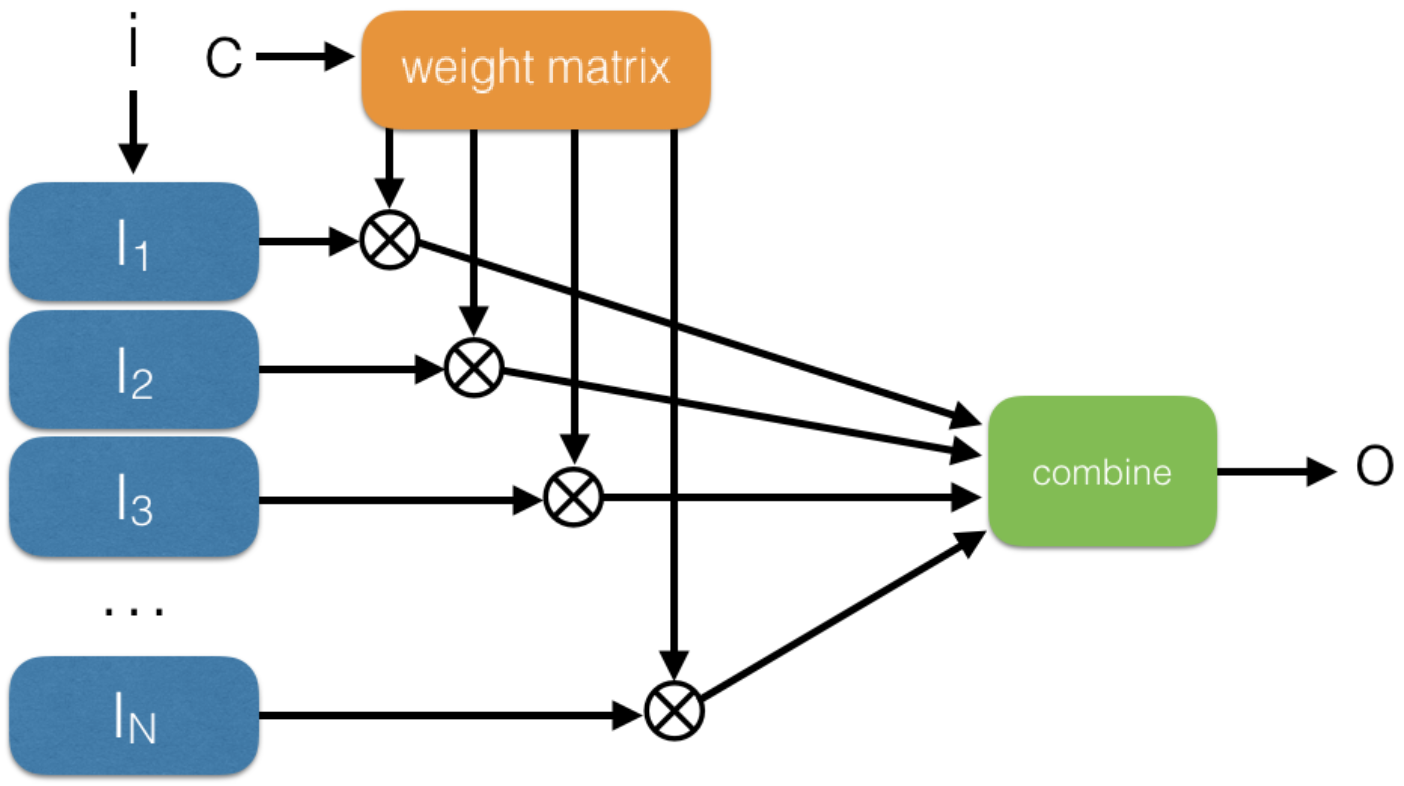
\includegraphics[width=0.4\linewidth]{./img/attention_gates.png}
                \end{figure}

                \begin{remark}
                    The gates of LSTM can be seen as attention mechanisms.
                \end{remark}


            \item[Squeeze and excitation] \marginnote{Squeeze and excitation}
                Layer that weighs the channels of the input through down-sampling and up-sampling.

                \begin{figure}[H]
                    \centering
                    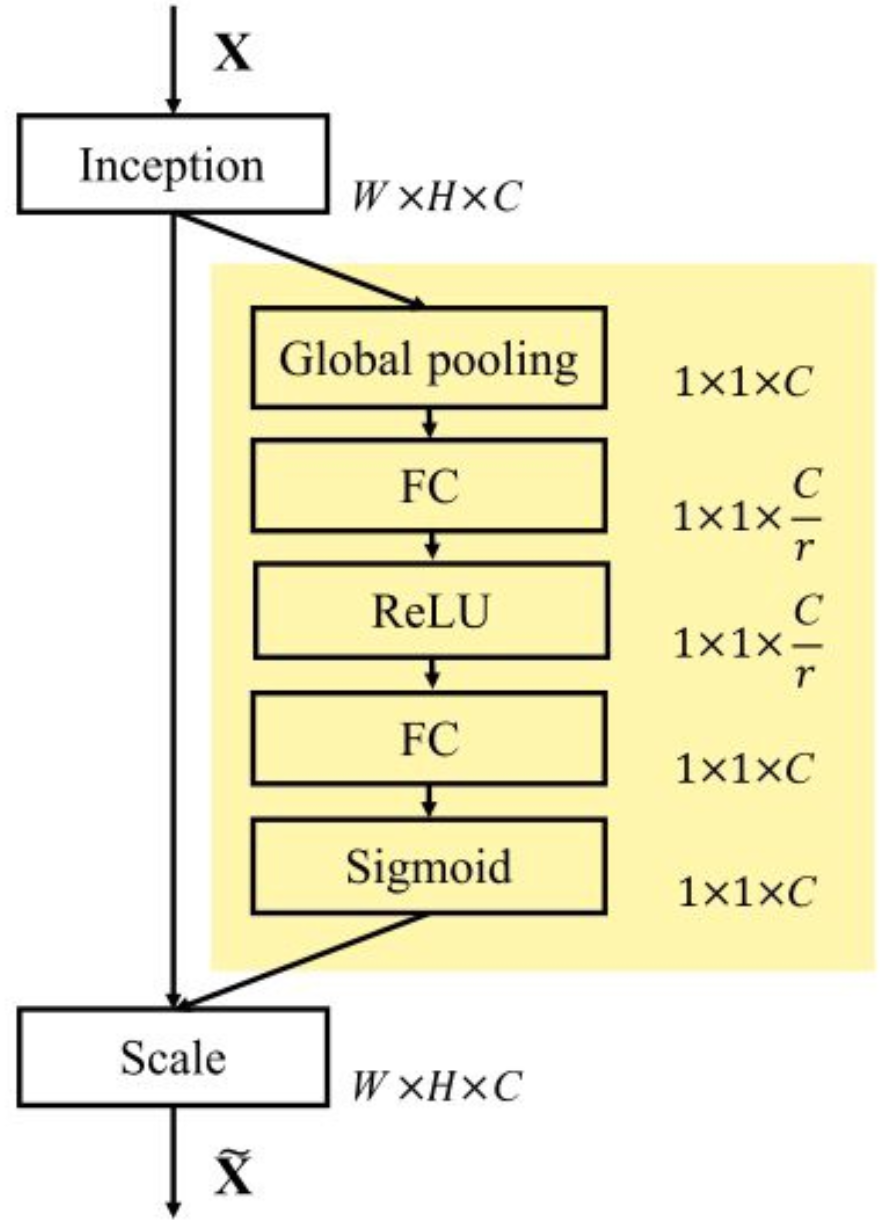
\includegraphics[width=0.25\linewidth]{./img/attention_se.png}
                \end{figure}

            \item[Key-value] \marginnote{Key-value}
                Generate an attention mask by comparing a query against some keys (which can be user-defined or learned parameters).

                Given a query $\vec{q}$ and $n$ keys $\vec{k}_i$ associated to $n$ values $\vec{v}_i$, 
                the score associated with each key is computed as:
                \[ \vec{a}_i = \alpha(\vec{q}, \vec{k}_i) \]
                where $\alpha$ is a score function. Commonly it can be:
                \begin{itemize}
                    \item The cosine similarity computed as the dot product: $\alpha(\vec{q}, \vec{k}_i) = \langle \vec{q}, \vec{k} \rangle$.
                    \item A single layer neural network: $\alpha(\vec{q}, \vec{k}_i) = \texttt{tanh}(\matr{W}_{\vec{k}_i} \vec{k}_i + \matr{W}_\vec{q} \vec{q})$.
                \end{itemize}

                The attention weights are obtained as:
                \[ \vec{b} = \texttt{softmax}(\vec{a}) \]

                Finally, the output is a weighted sum of the values:
                \[ \vec{o} = \sum_{i=1}^{n} \vec{b}_i \vec{v}_i \]

                \begin{figure}[H]
                    \centering
                    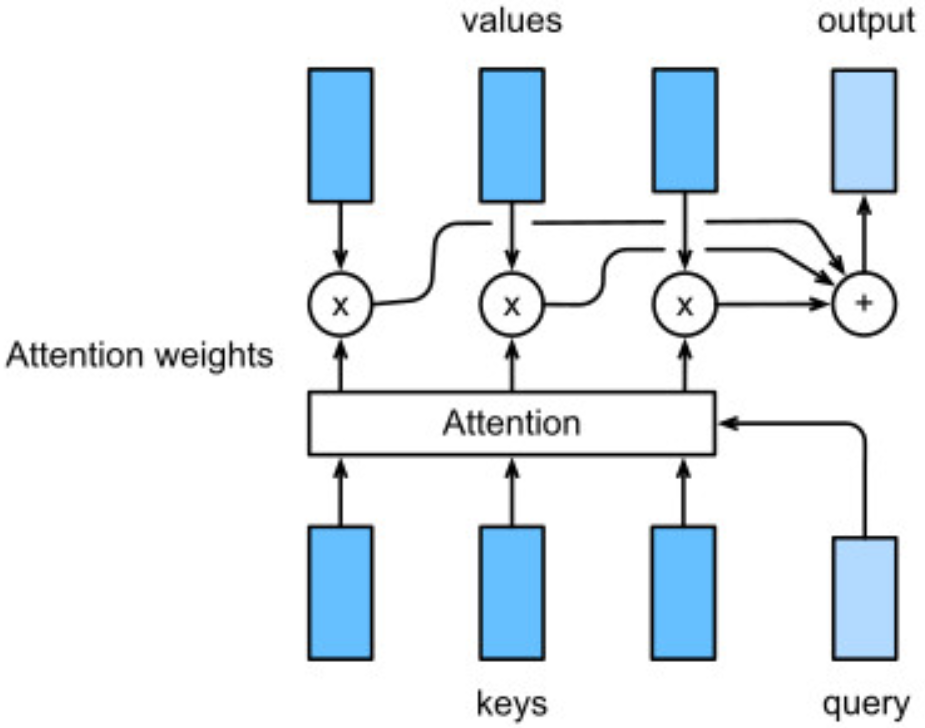
\includegraphics[width=0.25\linewidth]{./img/attention_key_value.png}
                \end{figure}

                \begin{description}
                    \item[Self-attention] \marginnote{Self-attention}
                        Case when values are also keys.
                \end{description}
        \end{description}

    \item[Transformer components]
        The main components of the Transformer architecture are:
        \begin{description}
            \item[Input and positional embedding] \marginnote{Embedding}
                The textual input is first embedded using a learned static embedding of size $d_{\text{model}}$ (i.e. mapping from token to vector).
                
                Additionally, as the model does not have recurrence, positional information is injected into the token embeddings (the original work uses sinusoidal functions).

            \item[Multi-head attention] \marginnote{Multi-head attention}
                Attention mechanism implemented using a key-value approach.

                Let:
                \begin{itemize}
                    \item $d_k$ be the size of the attention keys and queries,
                    \item $d_v$ be the size of the attention values,
                    \item $h$ be the number of heads of the multi-head attention mechanism.
                \end{itemize} 
                A single attention head computes the dot-product between queries and keys scaled by a factor of $\frac{1}{\sqrt{d_k}}$ to prevent the problem of vanishing gradient.
                In addition, queries, keys and values are projected using a learned linear transformation 
                (i.e. allow the model to learn the actual values of queries, keys and values to use).
                Therefore, a single attention head is defined as:
                \[
                    \begin{split}
                        \texttt{attention}(\matr{Q}, \matr{K}, \matr{V}) &= \texttt{softmax} \left( \frac{\matr{QK}^T}{\sqrt{d_k}} \right)\matr{V} \\
                        \texttt{head}_{i}(\matr{Q}_\text{in}, \matr{K}_\text{in}, \matr{V}_\text{in}) &= 
                            \texttt{attention}(\matr{Q}_\text{in}\matr{W}_{i}^\matr{Q}, \matr{K}_\text{in}\matr{W}_{i}^\matr{K}, \matr{V}_\text{in}\matr{W}_{i}^\matr{V})
                    \end{split}
                \]
                where:
                \begin{itemize}
                    \item $\matr{Q} \in \mathbb{R}^{\text{in} \times d_k}$, 
                        $\matr{K} \in \mathbb{R}^{\text{in} \times d_k}$ and 
                        $\matr{V} \in \mathbb{R}^{\text{in} \times d_v}$ are the matrices for queries, keys and values, respectively.
                    \item $\matr{Q}_\text{in} \in \mathbb{R}^{\text{in} \times d_{\text{model}}}$, 
                        $\matr{K}_\text{in} \in \mathbb{R}^{\text{in} \times d_{\text{model}}}$ and 
                        $\matr{V}_\text{in} \in \mathbb{R}^{\text{in} \times d_{\text{model}}}$ are the inputs of the head.
                    \item $\matr{W}_{i}^\matr{Q} \in \mathbb{R}^{d_{\text{model}} \times d_k}$, 
                        $\matr{W}_{i}^\matr{K} \in \mathbb{R}^{d_{\text{model}} \times d_k}$ and 
                        $\matr{W}_{i}^\matr{V} \in \mathbb{R}^{d_{\text{model}} \times d_v}$ are the learned projection matrices for queries, keys and values, respectively.
                \end{itemize} 

                The multi-head attention is defined as the concatenation of the single heads with an additional final projection:
                \begin{equation*}
                    \texttt{multi\_head\_attention}(\matr{Q}_\text{in}, \matr{K}_\text{in}, \matr{V}_\text{in}) = 
                        \texttt{concat}(\texttt{head}_{1}, \dots, \texttt{head}_{h}) \matr{W}^{O}
                \end{equation*}
                where $\matr{W}^O \in \mathbb{R}^{hd_v \times d_{\text{model}}}$ is the learned projection matrix for the output.
                
                Additionally, an optional mask can be applied to prevent future tokens to be accessed during training.

            \item[Feed-forward layer] \marginnote{Feed-forward layer}
                The feed-forward layer is simply composed of two linear transformations and an activation function (usually ReLU or its variants).
        \end{description}

    \item[Transformer] \marginnote{Transformer}
        Architecture composed of a stack of encoders followed by a stack of decoders.

        \begin{figure}[H]
            \centering
            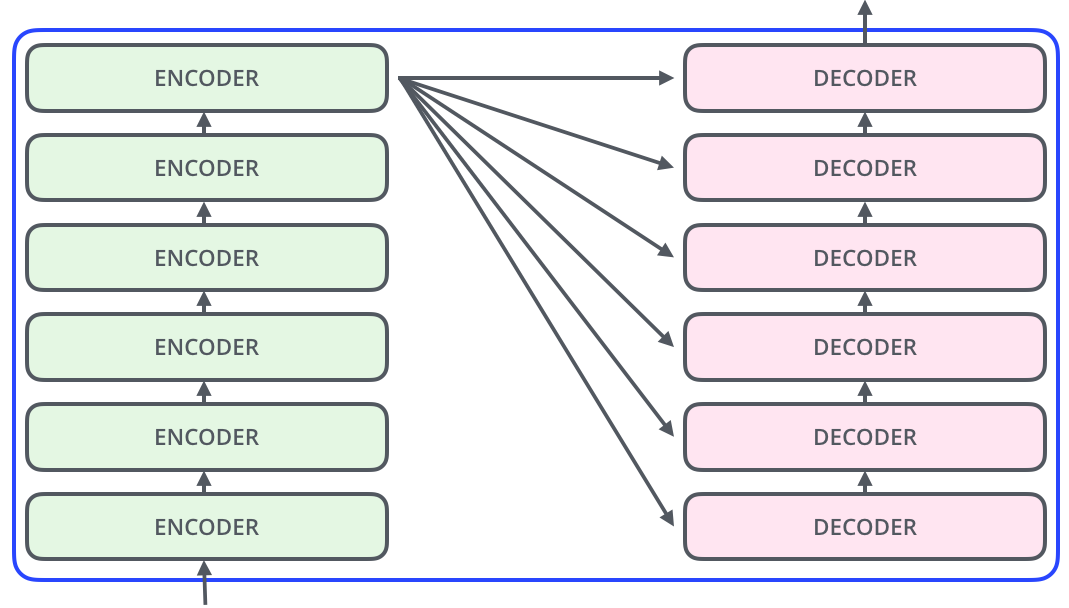
\includegraphics[width=0.35\linewidth]{./img/transformer_structure.png}
        \end{figure}

        \begin{description}
            \item[Encoder] 
                Extracts the relevant features of the input sequence.
                
                The first encoder receives the input sequence and the following ones take as input the output of the previous encoder.
                Each encoder is composed of:
                \begin{enumerate}
                    \item A multi-head attention that uses the input as query, keys and values.
                    \item A feed-forward layer.
                \end{enumerate} 

                The output of the encoder stack is passed to the decoders.

            \item[Decoder] 
                Auto-regressively generates the next token.

                The first decoder receives as input the token generated at the previous step (or a special initial token) 
                and the following ones take as input the output of the previous decoder.
                Each decoder is composed of:
                \begin{enumerate}
                    \item A multi-head attention that uses the input as query, keys and values.
                    \item A multi-head attention where 
                        keys and values are taken from the result of the encoder stack and the query is the output of the previous multi-head attention.
                    \item A feed-forward layer.
                \end{enumerate}

                The output of the decoder stack is passed through a softmax layer that returns the distribution for the next token.
        \end{description}

        \begin{figure}[H]
            \centering
            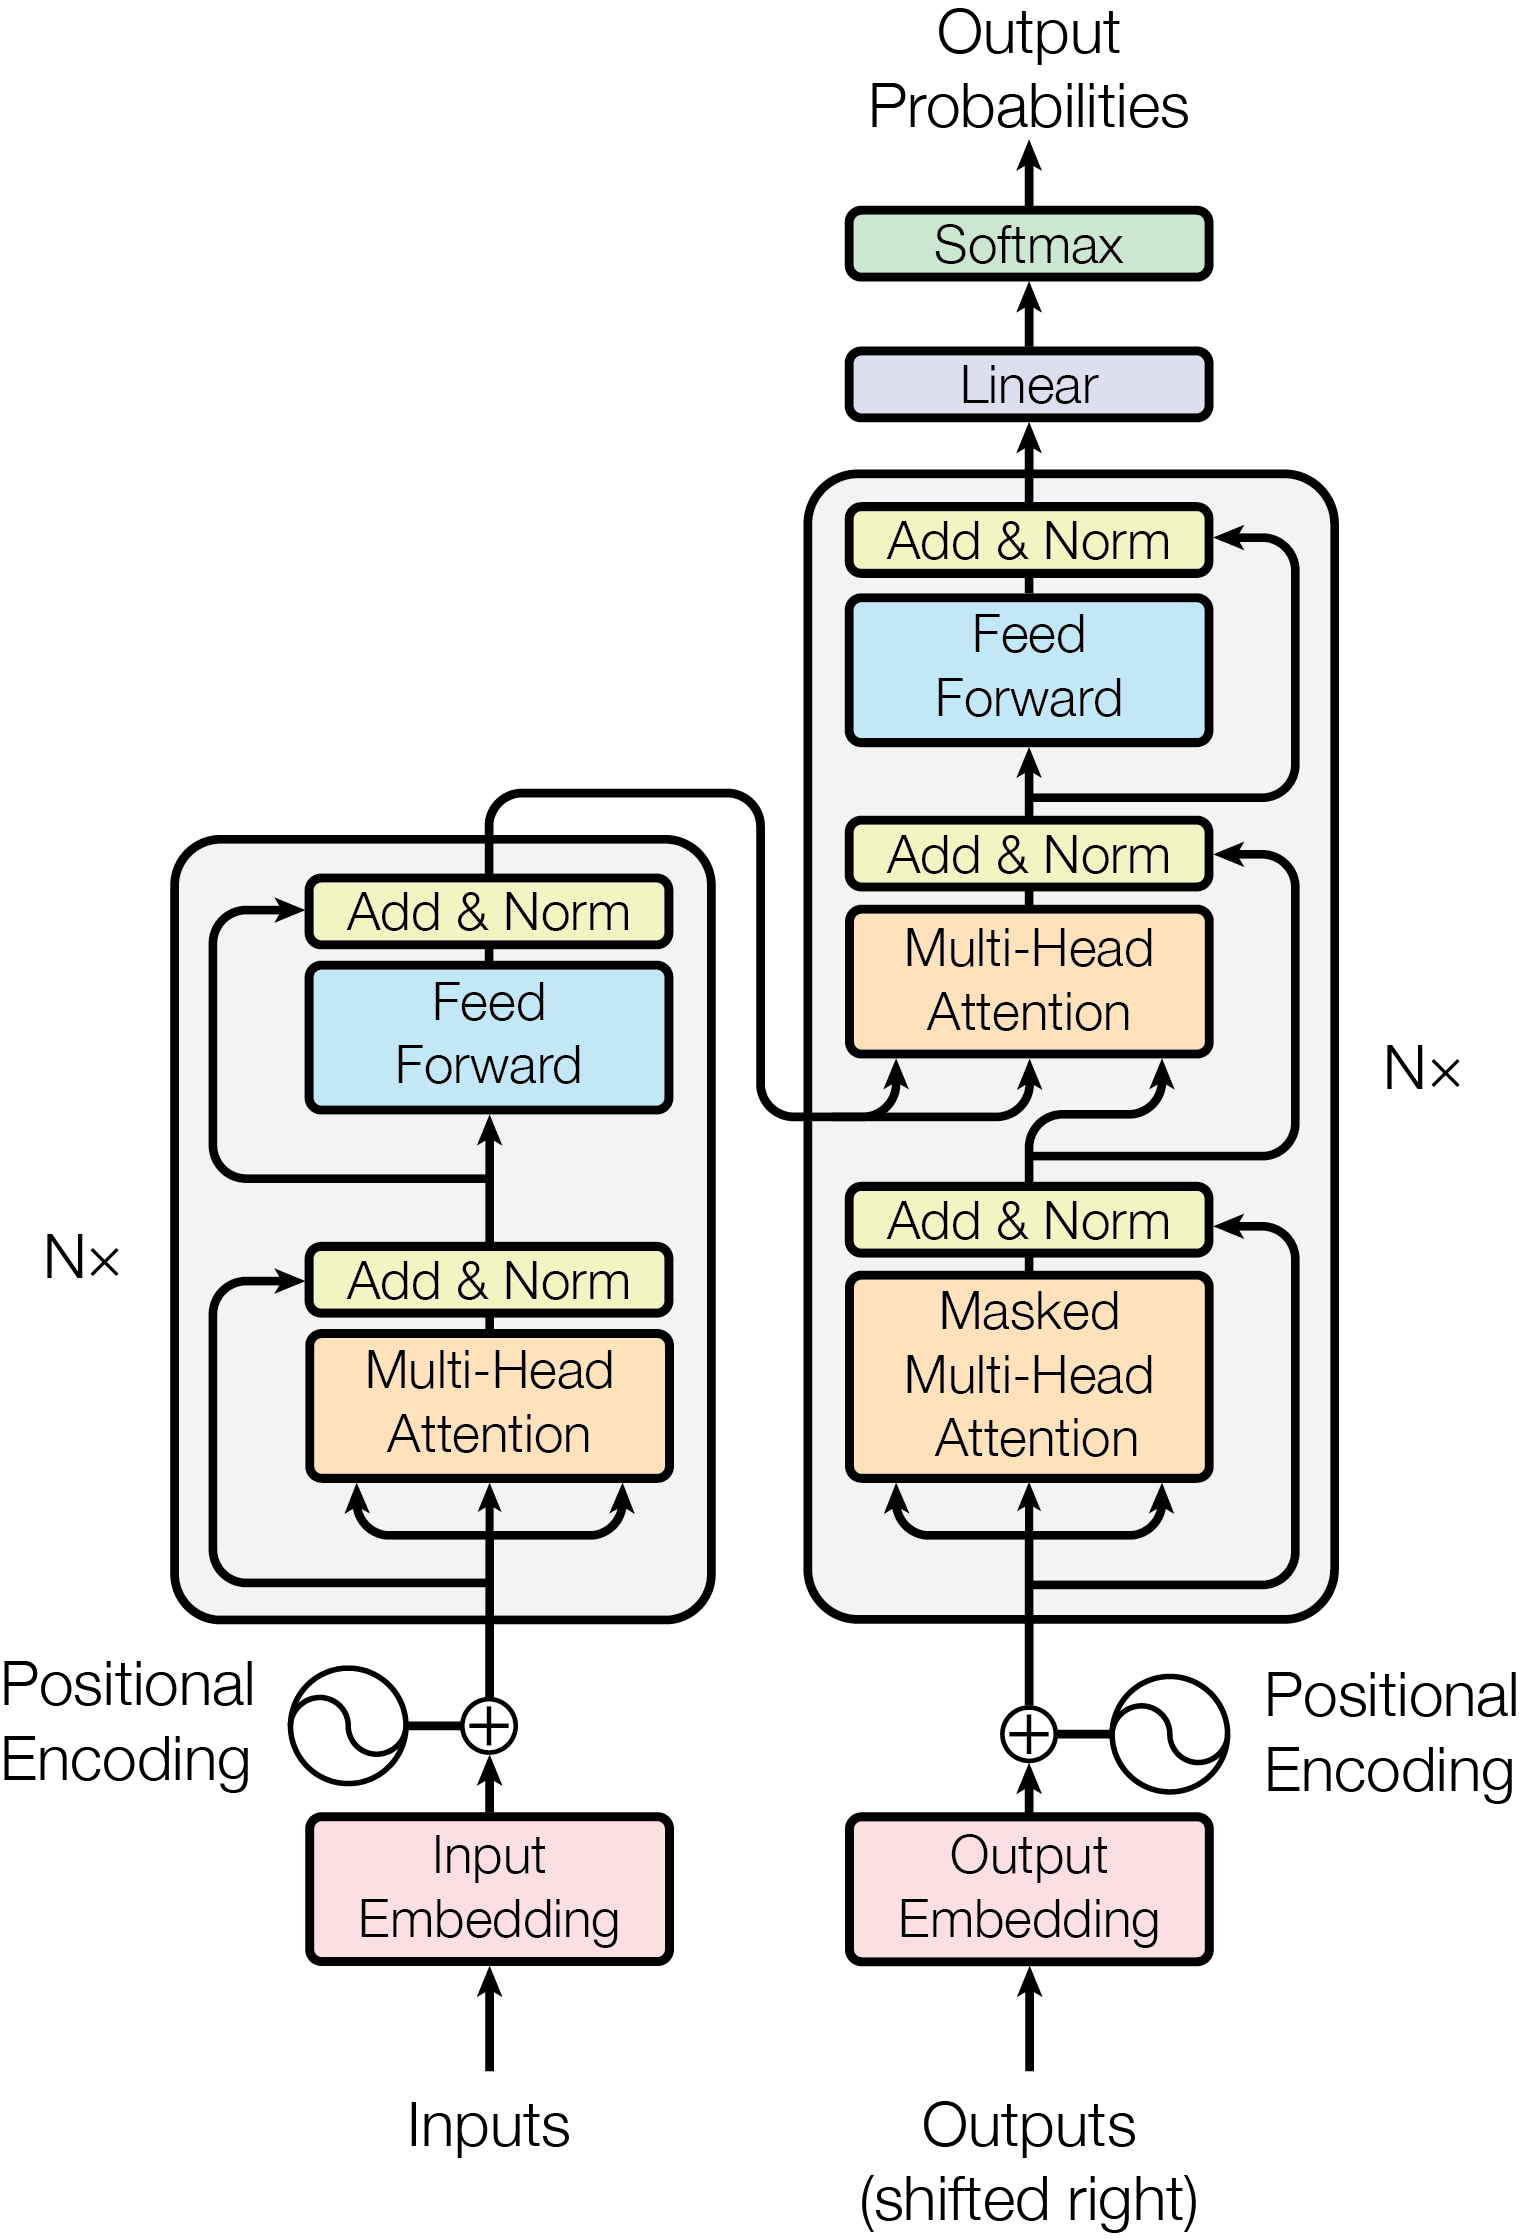
\includegraphics[width=0.35\linewidth]{./img/transformer.png}
            \caption{Compact representation of a Transformer encoder and decoder}
        \end{figure}

        \begin{remark}
            Depending on the architecture, only a part of the full architecture is used:
            \begin{descriptionlist}
                \item[Encoder-decoder]
                    Commonly used for sequence-to-sequence models where the input and output are both sequences (e.g. machine translation).
                
                \item[Encoder-only]
                    Suited for extracting features from the input sequence.
                    Usually used for classification tasks (e.g. BERT).
                
                \item[Decoder-only]
                    Used for auto-regressive models that are only able to attend at previously generated tokens.
                    Usually used for next token prediction (e.g. GPT).
            \end{descriptionlist} 
        \end{remark}
\end{description}
